
\documentclass[11pt]{article}
\usepackage{amsmath,amssymb,amsfonts} 
\usepackage{epsfig} \usepackage{latexsym,nicefrac,bbm}
\usepackage{xspace}
\usepackage{color,fancybox,graphicx,subfigure,fullpage}
\usepackage[top=1.25in, bottom=1.25in, left=1in, right=1in]{geometry}
\usepackage{tabularx} \usepackage{hyperref} 
\usepackage{pdfsync}
\usepackage[boxruled]{algorithm2e}
\usepackage{multicol}
\usepackage{enumitem}
\newcommand{\parag}[1]{ {\bf \noindent #1}}
\newcommand{\defeq}{\stackrel{\textup{def}}{=}}
\newcommand{\nfrac}{\nicefrac}
\newcommand{\opt}{\mathrm{opt}}
\newcommand{\tO}{\widetilde{O}}
\newcommand{\polylog}{\mathop{\mbox{polylog}}}
\newcommand{\supp}{\mathrm{supp}}
\newcommand{\rank}{\mathrm{rank}}
\newcommand{\ptot}{p_{\mathrm{tot}}}
\newcommand{\pmin}{p_{\mathrm{min}}}
\newcommand{\pmax}{p_{\mathrm{max}}}
\newcommand{\prob}[1]{\mathrm{Pr}\insquare{#1}}


\newcommand{\conv}{\mathrm{conv}}
\newcommand{\dist}{\mathrm{dist}}
\newcommand{\argmin}{\operatornamewithlimits{argmin}}
\newcommand{\sgn}{\mathrm{sgn}}
\newcommand{\fc}{\mathrm{fc}}


\newcommand{\cM}{\mathcal{M}}
\newcommand{\cB}{\mathcal{B}}
\newcommand{\cU}{\mathcal{U}}
\newcommand{\cY}{\mathcal{Y}}
\newcommand{\cF}{\mathcal{F}}
\newcommand{\capa}{\mathrm{Cap}}
\newcommand{\dcapa}{\underline{\mathrm{Cap}}}
\newcommand{\st}{\mathrm{s.t.}}
\newcommand{\un}{\mathrm{un}}

\newcommand{\Pb}{\mathbb{P}}
\newcommand{\sym}{\mathrm{sym}}
\newcommand{\pcount}{\mathbf{PCount}}
\newcommand{\mixdet}{\mathbf{MixDisc}}
\newcommand{\sbold}{\mathbf{S}}
\newcommand{\mb}{{M(\cB)}}

\newcommand{\mlb}{{M_{\mathrm{lin}}(\cB)}}
\newcommand{\redc}[1]{ \textcolor{red} {#1}}
\newcommand{\newt}{\mathrm{Newt}}
\newcommand{\wtf}{\widetilde{f}}
\newcommand{\wt}{\widetilde}
\newcommand{\diam}{\mathrm{diam}}
\newcommand{\lspan}{\mathrm{span}}
\newcommand{\interior}{\mathrm{int}}
\newcommand{\aff}{\mathrm{aff}}
\newcommand{\per}{\mathrm{per}}
\newcommand{\bl}{\mathrm{BL}}
\newcommand{\cE}{\mathbb{E}}


\newcommand{\eps}{\varepsilon}

\newenvironment{proof}{\noindent{\bf Proof:}\hspace*{1em}}{\qed\bigskip}
\clubpenalty=10000
\widowpenalty = 10000
\newcommand{\qed}{\hfill\ensuremath{\square}}


\def\showauthornotes{0} 
\def\showkeys{0} 
\def\showdraftbox{0}


\newcommand{\Snote}{\Authornote{S}}
\newcommand{\Scomment}{\Authorcomment{S}}

\newcommand\Z{\mathbb Z}
\newcommand\N{\mathbb N}
\newcommand\R{\mathbb R}
\newcommand\C{\mathbb C}

\newtheorem{theorem}{Theorem}[section]
\newtheorem{fact}{Fact}[section]
\newtheorem{conjecture}[theorem]{Conjecture}
\newtheorem{definition}{Definition}[section]
\newtheorem{lemma}[theorem]{Lemma}
\newtheorem{remark}[theorem]{Remark}
\newtheorem{proposition}[theorem]{Proposition}
\newtheorem{corollary}{Corollary}[section]
\newtheorem{claim}[theorem]{Claim}

\newtheorem{openprob}[theorem]{Open Problem}
\newtheorem{remk}[theorem]{Remark}
\newtheorem{example}[theorem]{Example}
\newtheorem{apdxlemma}{Lemma}
%\newtheorem{algorithm}[theorem]{Algorithm}
\newcommand{\question}[1]{{\sf [#1]\marginpar{?}} }

%% probability stuff

\newcommand\pr{\mathop{\mbox{\bf Pr}}}
\newcommand\av{\mathop{\mbox{\bf E}}}
\newcommand\var{\mathop{\mbox{\bf Var}}}

\newcommand{\ex}[1]{\av\left[{#1}\right]}
\newcommand{\Ex}[2]{\av_{{#1}}\left[{#2}\right]}

\def\abs#1{\left| #1 \right|}
\newcommand{\norm}[1]{\ensuremath{\left\lVert #1 \right\rVert}}



\newcommand{\tr}[1]{\mathop{\mbox{Tr}}\left({#1}\right)}
\newcommand{\diag}[1]{{\sf Diag}\left({#1}\right)}

\newcommand\set[1]{\left\{#1\right\}} %usage \set{1,2,3,,}
\newcommand{\poly}{\mathrm{poly}}
\newcommand{\floor}[1]{\left\lfloor\, {#1}\,\right\rfloor}
\newcommand{\ceil}[1]{\left\lceil\, {#1}\,\right\rceil}
\newcommand{\comp}[1]{\overline{#1}}
\newcommand{\pair}[1]{\left\langle{#1}\right\rangle} %for inner product
\newcommand{\smallpair}[1]{\langle{#1}\rangle}

\newcommand{\inparen}[1]{\left(#1\right)}             %\inparen{x+y}  is (x+y)
\newcommand{\inbraces}[1]{\left\{#1\right\}}           %\inbrace{x+y}  is {x+y}
\newcommand{\insquare}[1]{\left[#1\right]}             %\insquare{x+y}  is [x+y]
\newcommand{\inangle}[1]{\left\langle#1\right\rangle} %\inangle{A}    is <A>


\newenvironment{proofsketch}{\begin{trivlist} \item {\bf
Proof Sketch:~~}}
  {\qedsketch\end{trivlist}}

\newenvironment{proofof}[1]{\begin{trivlist} \item {\bf Proof
#1:~~}}
  {\qed\end{trivlist}}


\title{\bf CPSC 464: Modeling Alternative Affordable Housing Priority Systems}


\author{Andrew West, Nicole Lam, Atul Pokharel, Urszula Solarz \\
Professor: Nisheeth K. Vishnoi
}





\begin{document}


\maketitle
 
\begin{abstract}
Affordable housing is a widespread issue which pervades the United States. Yet, despite its magnitude, the system that each jurisdiction uses is quite opaque. Our project aims to fill this gap by leveraging publicly available data specific to Baltimore's low-income housing population. We intend to develop and implement a model that captures the dynamics of the housing allocation system by accounting for factors such as wait list turnover and applicant characteristics. Through this model, we will conduct simulations to predict how alternative priority systems might influence the demographic composition of housing recipients within Baltimore. Overall, we aim to provide a data-driven understanding of different affordable housing allocation strategies and their consequences on tenant demographics. We also assess the fairness and the impact through various empirically defined fairness metrics. 
\end{abstract}


\newpage



\tableofcontents

\newpage

\section{Introduction}
Housing is a basic necessity that is in increasingly scarce supply in American cities. One of the roots of this problem is that a full-time or 40-hour work week at minimum wage often cannot cover housing costs (\href{https://reports.nlihc.org/oor/connecticut}{NLIHC, 2019}). Therefore, many Americans turn to public, that is, government-owned housing. \\
\newline
The public housing ecosystem concerns five main agents: the federal government’s Department of Housing and Urban Development (HUD), municipal governments responsible for local housing policy, individual government-employees  responsible for implementing the housing allocation processes, beneficiaries currently living in public housing, and applicants on a waiting list. Secondary agents are private residents who are the face of movements like NIMBY and YIMBYism (Not/Yes in My Backyard), as well as PHIMBYism (Public Housing in My Backyard) which, though not the focus of this paper, affect potential public housing reform discussions. \\
\newline
As of 2023, around 11 million Americans rely on housing assistance or reside in public housing. 66\% of this population is made up of racial minorities, 32\% are female-headed families with children, and 35\% identify as disabled. \\
\newline
The application for housing support from the government often looks like the following portal for New Haven’s \href{https://elmcitycommunities.org/waiting-list/}{Elm City Communities}, where users are invited to join a waiting list. See Figure 1 for details.
\newline
\begin{figure}
    \centering
    
\includegraphics[width=0.75\linewidth]{elm.png}
    \caption{Example of Housing Portal}
\end{figure}
\\ Misalignment emerges in such an ecosystem as the group that makes decisions about the distribution of housing and what features necessitate prioritization, i.e. government and government agents, is not benefiting from it. A growing crisis ensues as demand continues to outweigh the supply of public housing, with no solution in sight. \\
\newline
Consider New York City, where there are around 200,000 public housing units for 400,000 people. 178,000 people are currently on the waiting list (\href{https://www.cbpp.org/research/housing/long-waitlists-for-housing-vouchers-show-pressing-unmet-need-for-assistance}{Acosta, 2021}). San Diego and Miami-Dade counties hold even longer waiting lists, with most US municipal housing agencies having 1,000+ families on their waiting lists for a median wait time of nine months (\href{https://nlihc.org/news/closed-waiting-lists-and-long-waits-await-those-seeking-affordable-housing-according-new-nlihc#:~:text=Public%20Housing%20provides%20homes%20for,average%20size%20of%20834%20households.}{NILHC, 2019}). Some factors that provide priority status for applicants on these waiting lists include income, age, and disability status. \\
\newline
Although the specific algorithms used to allocate affordable housing are not available, there appear to be two types based on whether or not the applicant is given any choice in the allocation. For example, after they are selected for housing by a lottery system, they may be presented with one or more options to choose from. Better under-standing how the presence of this choice can mitigate or exacerbate biases could help public housing authorities assess the fairness of allocation schemes currently in use, as well as enable citizens to hold governments responsible for fair allocations of a scarce, basic resource.\\
\newline
In general, there are two main modes of allocating housing to those who want it. One is the market mechanism in which those who can pay market price of housing receive it. A second one is through public housing agencies or similar non-market modes in which the cost of housing is significantly subsidized below market price. When there are fewer housing units than the number of those who want it and price cannot be used to allocate, who receives housing depends on an allocation algorithm. Some common algorithms for allocating housing in this latter scenario are lotteries and waitlists, with or without some other group-based preference ranking applied to it.\\
 \newline
There are two variations of non-market allocation algorithms depending on how much choice the recipient has. In the first, the recipient is presented with a choice of one or more units. They can either choose from among the set or choose to go back into the waitlist or lottery. While the fairness properties of different allocation schemes have been examined, to our knowledge, the fairness properties of allowing individuals to choose whether to accept or not is relatively understudied particularly in the presence of bias.\\
 \newline
While reversing the affordable housing crisis initially seems a problem unlikely to be solved in our generation, it is an urgent reality that must be confronted. The main case for it relies on the benefits of residential stability. \href{https://nhc.org/wp-content/uploads/2017/03/The-Impacts-of-Affordable-Housing-on-Health-A-Research-Summary.pdf}{Lubell, Crain, and Cohen (2021)} have previously presented the positive impacts of affordable housing on health. Furthermore, secure housing also improves education outcomes by reducing high household mobility, of which the US has the highest rate across developed countries; there is a strong, negative relationship between such frequent residential mobility and educational performance. Lastly, in response to the argument that affordable housing threatens neighborhood property values,  \href{https://www.researchgate.net/publication/235355600_Affordable_Housing_Reader}{ Mueller and Tighe (2012)} demonstrate the community wide benefits of affordable housing.\\
\newline
There is widespread precedent in Europe that discussions on public housing reform can be destigmatized and the option be turned into a norm. For instance, in Vienna, 60 percent of the population lives in non-market housing in a broader integrated unitary housing market (\href{https://www.researchgate.net/publication/341951502_How_Much_State_and_How_Much_Market_Comparing_Social_Housing_in_Berlin_and_Vienna}{Glaser, 2020}). Similarly, Amsterdam's 30\% non-market housing is considered a middle class subsidy, not a government handout (\href{https://www.jchs.harvard.edu/blog/peoples-housing-non-profit-social-housing-netherlands}{Van Deursen, 2023}).\\
\newline
There are two significant bottlenecks in the United States that have previously prevented larger action on this issue that could lead to similar outcomes as in Europe. The first is a legislative measure; while some people may argue that this supply-side problem can be solved by building more public housing units, this is not legally possible due to oft-recurring challenges like the Nixon-era construction moratorium and Clinton Faircloth Amendment to the 1937 Housing Bill (\href{https://www.hud.gov/sites/documents/FRCLTH-LMT.PDF}{HUD}). The second concerns limited representation at City Council meetings across the nation whose inconvenient meeting times and lack of principled approach often lead to exclusions of certain populations (\href{https://www.ncbi.nlm.nih.gov/pmc/articles/PMC8149917/}{McNee et Pojani, 2021}). Other related barriers include exclusionary zoning and parking requirements (\href{https://www.brookings.edu/articles/the-double-edged-sword-of-upzoning/#:~:text=Cities%20are%20in%20desperate%20need,contributes%20to%20rising%20housing%20costs}{Davis, 2021}).\\
\newline
The work of this paper will be twofold: first, we aim to model the existing conditions of our chosen city's public housing allocation, followed by assessing new queue and priority systems and examining their effects on the demographics of those we predict will be offered public housing. Figure 3 shows these main tasks and contributions.\\
\begin{figure}
    \centering
    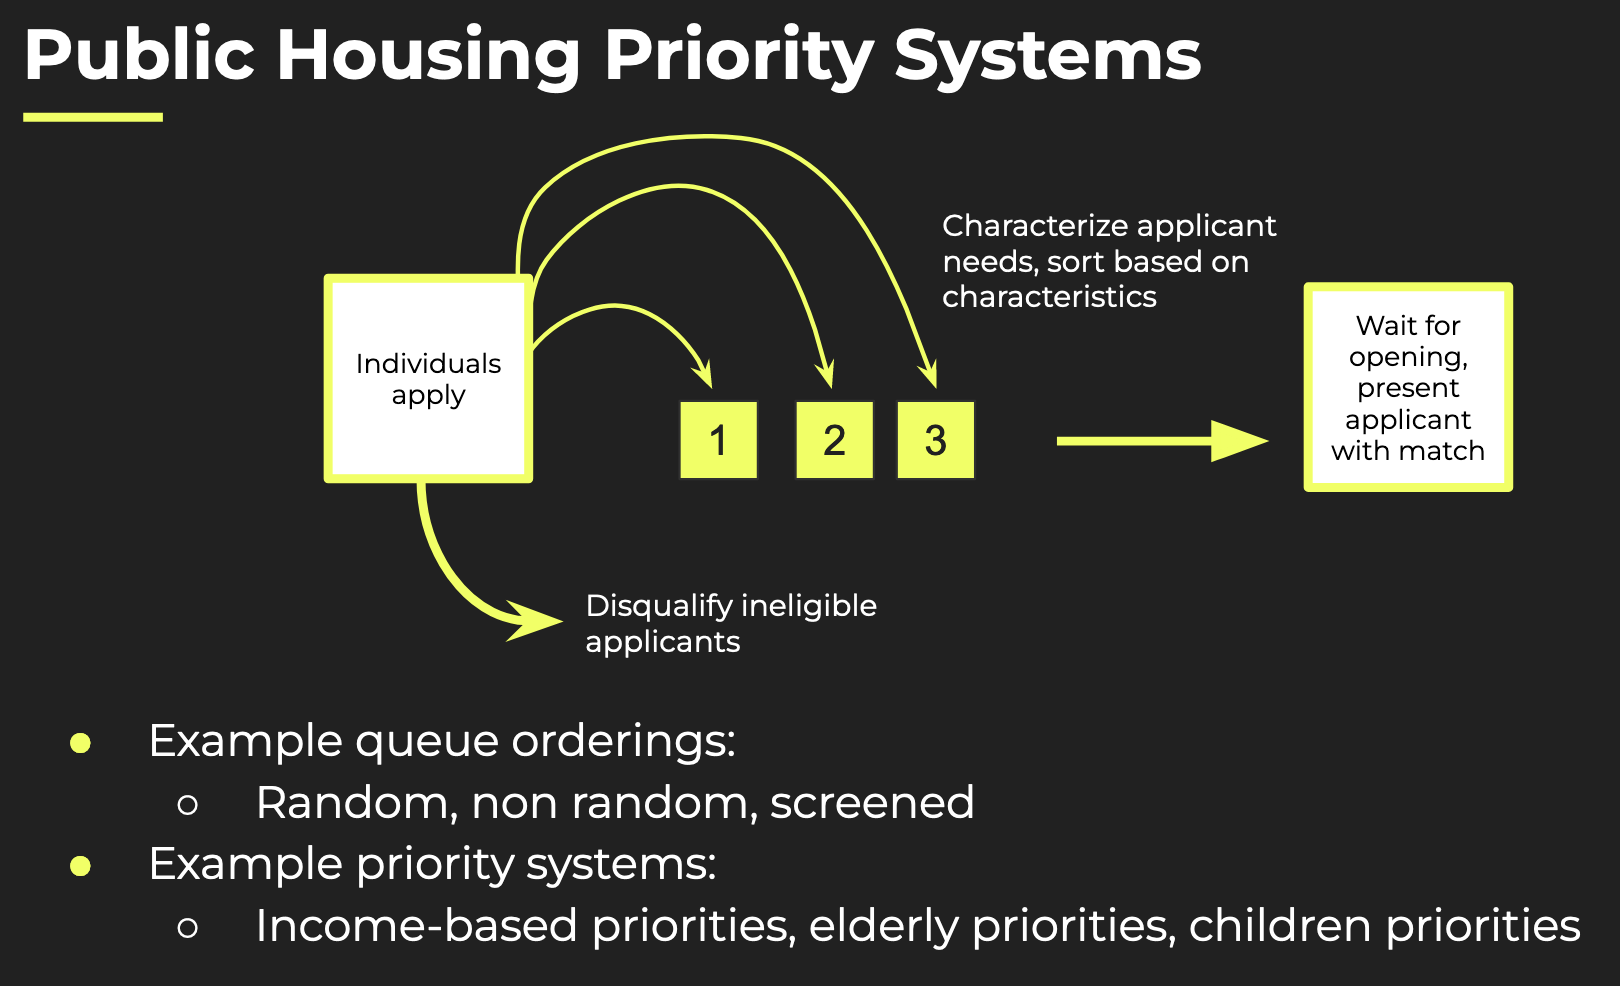
\includegraphics[width=0.75\linewidth]{schematic_priority _systems.png}
    \caption{Diagram of public housing allocation systems}
    \label{fig:schematic}
\end{figure}
\newline
Little is typically known about the methods that cities use to allocate public housing, meaning our first task is to model this process. Using publicly available data on who is awarded housing, we can estimate this process for our chosen city. Relying on estimations made by previous works, we can also integrate assumptions about the rate at which housing becomes available into our predictions to gain a comprehensive approximation of overall public housing availability and allocation. We can apply this model to our city of choice to estimate the flow of applicants in, through, and out of public housing under the city's current system. \\
\newline
With an established model for the present conditions of a city, we can proceed to evaluate alternative allocation systems for fairness. We will apply these alternative systems to our model in order to comment on how the characteristics of tenants shift with the goal of informing future decision making in this sphere. This makes use of a conceptual novelty, in that we expect that ours will be one of the few empirical examinations of fairness implications of choice in housing allocation schemes, as well as a technical novelty in that we will have to develop novel means of approximating allocation mechanisms.
\section{Other related works}
The allocation of scarce resources is a classic problem that pervades social service delivery. At the highest level, prior research has examined the necessity of trade-offs for fairness in social contexts \cite{mashiat2022trade}, arguing that often times many reasonable definitions of equity cannot hold simultaneously. This paper in particular creates a metric of fairness to analyze average realized utility of a resulting outcome, but does not give way to implement allocation systems, which we wish to examine. \\
\newline
There are a variety of studies regarding affordable housing and approximating allocation algorithms. The major limitation of all these studies is that the algorithms are not public. However, Figure 2 describes the general stages of any scheme.\\
\newline
Some papers have abstracted the problem of housing allocation into that of designing waitlists and lotteries \cite{arnosti2020design}. They claim that two approaches of housing allocation create near-optimal matches: independent lotteries and waitlists. They examine in great detail these two modes of allocation, but does not examine the inherent factor of consumer choice in the housing allocation process. Another paper addresses this shortfall by implementing a modified version of the latter of these systems on housing data from Pittsburgh \cite{harvardpublichousing}. Specifically addressing the issue of allocation inefficiency, they argue that implementing an independent waitlist per building reduces the amount of vacant buildings emptied during turnover. However, this algorithm does not account for the nuances of household differences (size, number of children/elderly, veteran status...), which is what we intend to explore. \\
\newline
In our project, we aim to analyze the demographic effects of tenant populations by changing the order of allocations, as in \cite{nyuaffordablehousing}. This paper tackles the issue that housing allocation methods are often unknown and opaque. Thus, they created an algorithm to include priority systems (moving populations with certain characteristics to the front of a queue). Specifically, they analyzed the changes in tenant composition by prioritizing high income households, low income households, the elderly population, and families with children under 18. While the model does shed light on the magnitude of change in these particular orderings, it limits the eligible applicants to those whose household income is above 80\% of the area median income, which severely skews the results. There are also many other key variables such as families with victims of domestic violence, military status, and veteran status that were not explored.\\




\section{The Model/Framework}
\noindent
Our city of choice to model policy changes is Baltimore. With a population of close to 600,000 and a public housing system containing approximately 6,000 properties, Baltimore's robust and widely used public housing system is an ideal choice for analyzing the impacts of differing priority systems on allocation outcomes. \\
\newline
Demand for public housing in Baltimore is also exceedingly high. The public housing system lottery opened for the first time since 2019 this August, with nearly 30,000 applicants applying during the two week window (\href{https://www.wypr.org/wypr-news/2023-08-14/28-000-apply-for-baltimore-city-housing-wait-list-two-week-window-ends-tonight}{Baltimore WYPR}). Priority systems are unfortunately essential to best allocate the limited available housing to those most in need. \\
\newline
Baltimore is also an ideal choice due to the availability of relevant datasets, discussed further in 6.1. \\
\begin{figure}
    \centering
    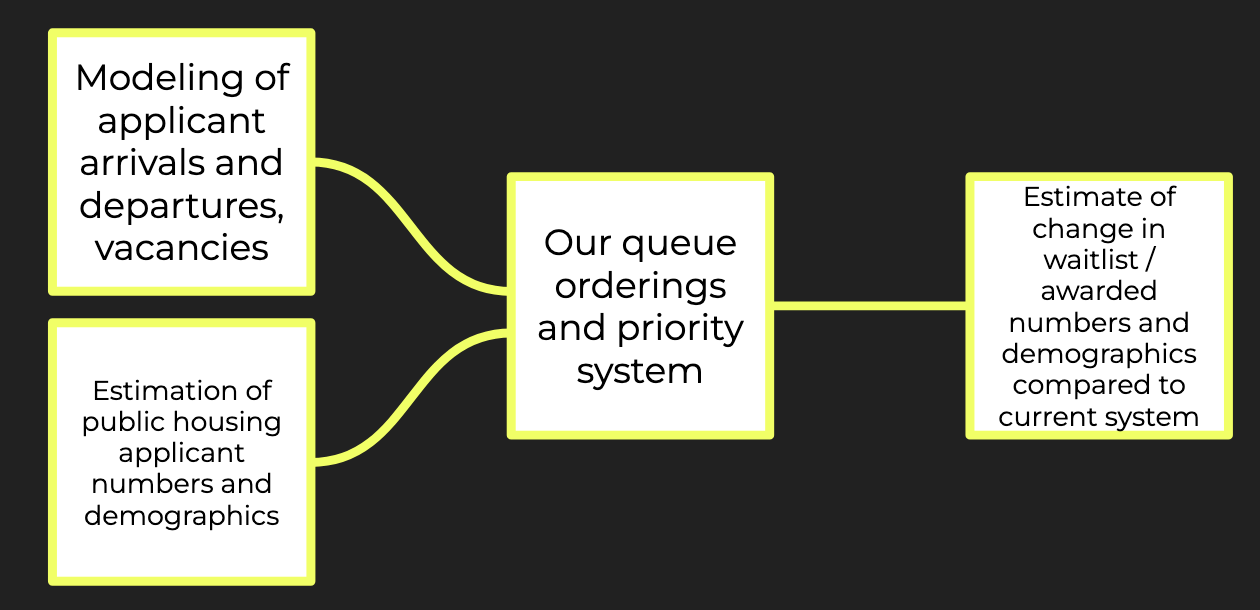
\includegraphics[width=0.75\linewidth]{ourmodel.png}
    \caption{Proposed model of our contributions}
    \label{fig:enter-label}
\end{figure}
\\Our model (see figure 3) includes multiple components due to the complexity of applicant selection that takes place in public housing allocation. Broadly, the framework is as follows:
\begin{enumerate}
    \item Estimate who is eligible for Baltimore public housing, and of the eligible pool, who applies.
    \item Estimate the existing allocation system.
    \item Implement changes in housing priority systems and other waitlist variables to model the effects when compared to actual waitlist demographics. 
\end{enumerate}
Modeling the waitlist and how it changes under new policies also requires us to consider the human factors that impact waitlist membership. In particular, we will make assumptions about the rate at which applicants apply, any applicants that leave the waitlist, and the rate at which apartments become available for new occupants.
\subsection{Various Housing Allocation Algorithms}
As forementioned in our prior related works section, we know very little about the methods jurisdictions use to allocate assistance. One such paper attempts to approximate the different algorithms of housing allocation systems deployed in different cities. The steps are detailed below:
\begin{enumerate}
    \item Households successfully complete the application for housing assistance. Many eligible households don't apply for assistance due to lack of functioning abilities, language skills, or other tools needed to complete the application.
    \item Applications are deemed eligible or non-eligible (income greater than 80\% of average median income to apply, employment, geographic location, etc.)
    \item Categorize the various characteristics for each household applicant (unit size, military status, number of children, income level, etc.)
    \item Match type of housing (1-bedroom, 2-bedroom, etc.) with each household applicant based on their characteristics in step 3
    \item The order in which applicants will receive allocations for each housing type is determined (i.e. random lottery, first come first serve queues, some metric of ``need", or a combination)
    \item Present chosen applicants with at least one available housing option. In some cases, applicants apply only for a particular housing development in some location, so they must take the option or leave the queue (or allocation system) all together. Other systems allow applicants to reject the particular unit or development, but stay in the queue for other, more desirable, units that become available.
\end{enumerate}
\subsection{Cambridge Housing Model}
\label{sec:chm}
In the same paper, the author attempts to examine the specific housing system of one Public Housing Agency: the Cambridge, MA Public Housing Agency (CHA) at a specific point in time (2012 calendar year) \cite{nyuaffordablehousing}. To model the public housing waitlist run by the Cambridge Housing Authority, we define the following variables: (1) how frequenctly new applicants arrive on the waiting list, (2) when public housing apartments become available, and (3) when applicants depart from the waiting list without being assigned housing. \\
\begin{itemize}
    \item \textbf{Applicant Arrivals Rate}: Suppose that applicants for public housing arrive on the waitlist at rate $\alpha$, which we define as poisson. In other words, the number of arrivals follows a Poisson distribution with $\alpha$ expected annual arrivals. The model chooses arrival rate to be constant over four year increments. Though, it also notes that this arrival rate may vary more frequently(daily, uniform annually, uniform over two years). 
    \item \textbf{Public Housing Vacancy Rate: } Next, suppose that apartments of type $k$ become vacant at rate $v_k$. There are two methods by which $v_k$ can increase: tenants vacating their units or increased stock in public housing. The model assume that the vacancy rate remains relatively constant.
    \item \textbf{Applicant Departure Rate: } Represent the rate that applicants leave the waitlist without housing as $\delta$. The model assumes that each applicant has an equal probability of departing from the waitlist. Meaning, each applicant departs the waiting list at some random, unpredictable date. The model describes that the time of departure is modeled with an exponential distribution with parameter $\delta$.
\end{itemize}
Next, the model then overlays the aspect of household preferences on top of this waitlist model. More specifically, the model creates two queues for each development type: a high-priority queue $i$ and a low priority queue $j$. Let us denote the wait time for these queues as $T_i$ and $T_j$. Then, the model claims that the wait time of these queues are zero, positive, or infinite. More specifically, every member of $T_i$ must be matched before any member of $T_j$ can be considered. In other words, if $T_i \neq 0$, $T_j = \infty$. 
\section{(Desired) Theoretical results}
We are still at the early stages of performing empirical experiments using our code. It is unclear what theoretical results might emerge once we are able to look at how different fairness measurements change across allocation type. 
% \subsection{Preliminary results}

\section{(Desired) Empirical results}

\subsection{Setup}
\paragraph{Datasets.}
Our work will employ three datasets. The first is the \href{https://data.census.gov/mdat/#/search?ds=ACSPUMS5Y2021}{American Community Survey (ACS) microdata}. The ACS is an annual survey conducted with the aim of being a nationally representative sample of demographic, economic, and housing information. We will employ demographic variables contained in the ACS data to estimate the number of households elligible for public housing. \\
\newline
Our second dataset is the \href{https://www.huduser.gov/portal/datasets/assthsg.html}{HUD’s Picture of Subsidized Households (PIC) data}. The PIC data contains information on demographics of public housing tenants, public housing vacancy rates, and average waiting times that will be helpful in constructing our model. \\
\newline
Finally, we will make use of the \href{https://www.hud.gov/sites/dfiles/PIH/documents/BaltimoreFY20Report.pdf}{2020 Baltimore public housing waiting list demographics}. This information will allow us to validate our model of the existing allocation system.

\paragraph{Algorithms}
Using the Cambridge housing allocation model in section~\ref{sec:chm}, and the data for Baltimore, we will simulate the waitlist (likely using C). We will run each simulation for a fixed number of iterations, $N$. At the end of $N$ iterations, we will measure the fairness of the resulting allocation using each of the metrics below. After $M$ runs of this simulation we will be able to obtain an empirical distribution of each of the fairness metrics below. \\
\newline
The Cambridge model is a simple waitlist with priorities but without choice. To incorporate priorities we will use $n+1$ queues for each waitlist given $n$ priority groups. 
When a vacancy opens up, everyone in a higher priority group is offered the housing before those of the next group. \\
\newline
Third, to model choice we will introduce a variation of each of the above two types of waitlists (with and without priority). There are two forms of choice relevant here. First is the submission of a list of preferences across housing developments for each applicant. The second is to permit the matched applicant the option to decline the offer and return to the queue. We will include each of these in our later models, and assume that the likelihood of each choice comes from a distribution of our choice. 
\paragraph{Baselines and metrics}
The baseline model is the Cambridge model above. As we change the parameters of our simulation runs, we will measure the outcomes against that. We will use the following list of fairness metrics to assess the resulting allocations. 
\\
\\
Let $G_1, G_2, \dots, G_\ell$ be subsets of our data. Let $n_k$ be the number of people chosen in the $k$-th subset. Furthermore, for every $X \in G_k$, let $X=(S_k, N_k)$ represent the socially-salient, and non-socially-salient attributes, respectively. Lastly, assume that $Y$ is a true equilibrium and $\hat{Y}$ is our predicted equilibrium.
\begin{table}[h]
    \centering
    \begin{tabular}{c|c}
        Fairness Metric & Description \\
        \hline
         Group Fairness (Equality) & $n_i = n_j$ for $i \neq j$ \\
         Group Fairness (Proportional) & $n_i / |G_i| = n_j / |G_j|$\\
         Group Fairness (Range) & $n_i \geq c \cdot n_j$ where $c \in [0,1]$ \\
         Fairness Through Unawareness & $\text{minimize}(N_i - N_j)$ for $|\hat{Y}_1 - \hat{Y}_2| \rightarrow 0$ \\
         Outcome Dependent Fairness (Separation) & $\hat{Y}$ does not depend on $S$ given $Y$ \\
         Outcome Dependent Fairness (Sufficiency) & $Y$ does not depend on $S$ given $\hat{Y}$ \\
         Outcome Independent Fairness & Relaxing Statisical Parity: $\frac{P(\hat{Y} = 1 \mid S = i)}{P(\hat{Y} = 1 \mid S = j} \geq 1 - \epsilon$ 
    \end{tabular}
    \caption{Fairness Metrics and Descriptions}
    \label{tab:fairness_metrics}
\end{table}
Algorithms naturally encode human biases, so having an empirical set of fairness definitions provides a testing regime for how our proposed ranking system compares to others. These definitions are a more reliable metric than simply assuming diversity implies fairness. 

\section{Next Steps, Limitations, and Future Work}
A particularly salient area of future research considers consumer choice after considering the utility (perceived and actual) of their allocated public housing unit. This is useful in further making the ranking system more fair and efficient, so that more families accepts their initial housing draw – that is, through maximizing utility, each applicant(s) should be matched with housing that most suits their preferences so they don’t take up space for multiple units, or have to return to the waitlist after being being matched with an unsatisfactory unit. \\
\newline
In the past, families have been actively encouraged to apply to units in multiple locations to maximize their overall chance of being matched with housing. Though the average number of housing applications an American family submits is unknown, housing portals state, “The more lists you’re on, the higher your chances of being awarded a housing choice voucher” (\href{https://benefits.com/section-8/waiting-list/#:~:text=You%20can%20also%20apply%20with,awarded%20a%20housing%20choice%20voucher.}{Benefits.com}). This complexity has contributed to an increasing amount of time between tenants as agencies simultaneously hold different units for the same person, who will, ultimately, only choose the best unit. This extends the waiting time for everyone as that same applicant gets screened and contacted (both being time-intensive processes) for each of the various units they applied for. The Agawam Housing Authority in Massachusetts, for instance, reports that it takes years to find a new tenant, as hundreds of names must be analyzed before a match is found (\href{https://www.wbur.org/news/2023/09/19/massachusetts-state-funded-public-housing-waitlist-vacant}{Wallack \& Willmsen, 2023}). Scenarios like this result in phenomena like in the nearby town of Gardner, Massachusetts which has a vacancy rate of 21\%, meaning 70 out of 342 units are vacant even as the waitlist contains 11,775 people (\href{https://www.wbur.org/news/2023/09/19/massachusetts-state-funded-public-housing-waitlist-vacant}{Wallack \& Willmsen, 2023}). On a national scale, the \href{https://www.google.com/url?q=https://www.hud.gov/program_offices/public_indian_housing/programs/ph/PH_Dashboard?utm_medium%3Demail%26utm_source%3Dgovdelivery&sa=D&source=docs&ust=1697432365239122&usg=AOvVaw2yT-DQb6XprsdCaD2vsE1k}{Public Housing Dashboard put out by the HUD} reveals that there is a lesser, though still significant vacancy rate of five percent. Northwestern states like Oregon, Washington, and Idaho have higher-than-average occupancy rates while Kansas and Maryland have sub-90\% occupancy rates. All things considered, having any vacant unit can be considered a failure of the matching algorithm and have significant societal implications. \\
\newline
While determining if an algorithm maximizes utility initially seems like an especially useful mechanism for evaluating an algorithm’s fairness, it comes with certain drawbacks and limited technical feasibility. The first is that it, like many other fairness measures, relies on highly accurate data. However, inaccuracies can arise through human data entry leading to incorrect documentation of familial characteristics (e.g. number of children) or lack of up-to-date information on the state of or vacancy of housing (e.g. whether or not it is occupied or under renovation, thus unavailable). The curation of the former and maintenance of the latter is resource-intensive from a financial and human capital perspective. \\
\newline
Further bias can arise from the assumption that certain familiar characteristics align with preference for certain housing, i.e. assuming that families with more children prefer larger housing units. If an empirical way to collect these preferences is indeed established, it has to account for context drift or familial circumstances and preference changing over prolonged waiting times \cite{conceptdrift}. \\
\newline
In conclusion, these obstacles serve as a reminder that the design of algorithms is intrinsically linked with human decision-making and subjectivity \cite{humanerror}. Technical improvements and considerations of the societal implications of the algorithms used in housing policies are only part of the process of ensuring fairer housing allocation in places like Baltimore. After all, historic housing policy decisions play a leading part in dictating the effectiveness of current policy efforts. We hope this paper encourages broader and more thoughtful discussion on the usage of computer science in improving the lives of urban dwellers. 

\newpage
\section{Appendix 1: Data Prep Scripts}
.do files prepare the data. Filenames in bold are not generated by the scripts. They have to be available to them instead. Each of the scripts is described below.

\subsection{ACS-extract.do}
Input: \textbf{data/ACS/usa\_00003.dat/usa\_003.dat} \\
Output: data/ACS\_2006\_2017.dta \\
Guess: This looks like American Community Survey (ACS) data from 2006 to 2017. \\
Source: 

\subsection{descriptives-CHA.do}
Input: data/Matlab/eligible\_population\_CHA.dta \\
Output:  results/Descriptive/ \\
- acs\_descriptive\_CHA.dta \\
- descriptive\_table\_auto.xls  (with sheets “ACS All”, “ACS by Type” )\\
		- acs\_descriptive\_CHA\_bytype.dta\\
		- pic\_descriptive\_CHA.dta\\
		- descriptive\_table\_auto.xls ( with sheet "PIC All" and "PIC by Type" )\\
		- pic\_counts\_CHA\_bytype.dta\\

\subsection{eligible-population.do}
Input: data/\\
ACS/ACS\_2006\_2017.dta\\
\textbf{other/ami.dta}\\
Output: data/Matlab/ \\
- eligible\_population\_CHA.dta\\
- eligible\_population\_CHA.txt (A pipe delimited file)

\subsection{pic-data.do}
Input: data/ \\
\textbf{HUD-PIC/2012/PROJECT\_2012.csv} \\
\textbf{other/CHA-projects.csv} \\
Output: \\
data/ \\
- HUD-PIC/2012/PIC-CHA.dta \\
- Matlab/projects-ready.dta \\
- Matlab/projects-ready.txt \\
- other/waiting-times-CHA.dta\\
results/descriptive/ \\
-   pic\_by\_development.dta \\
- development\_characteristics.xls ( with sheet("raw") ) \\

\section{Appendix 2: Primary Datasets}
The data processing pipeline is shown in Figure~\ref{fig:datapipeline}. The primary files are underlined in red  and described below. See this \href{https://docs.google.com/spreadsheets/d/1rT5IQdjf1eXFhCbJFr7dV0yZLzTJhNmbBcI5qajiMEw/edit#gid=555949214}{associated  spreadsheet} for the fields and below for any additional notes. The relative files are:

\begin{figure}
    \centering
    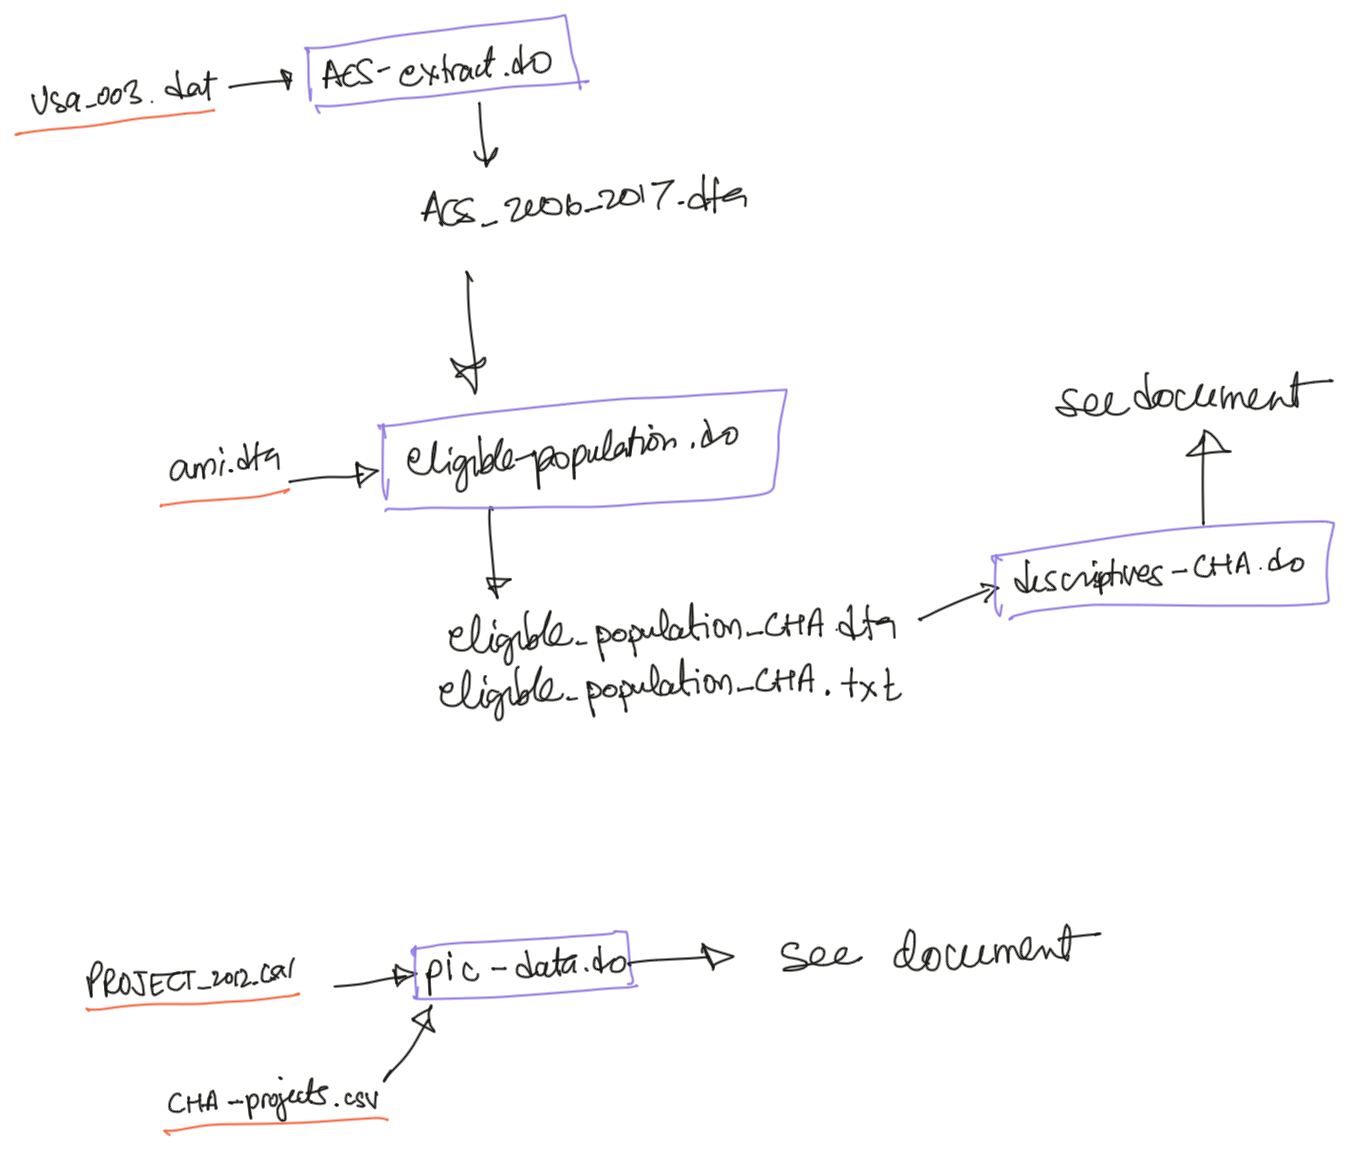
\includegraphics[width=1\linewidth]{doc/data_processing_pipeline.png}
    \caption{Data processing pipeline. Primary data is underlined, and scripts are in purple boxes. Arrows denote input or output.}
    \label{fig:datapipeline}
\end{figure}
\begin{itemize}
    \item usa\_003.dat
    \item ami.dta
    \item PROJECT\_2012.csv
    \item CHA-projects.csv
\end{itemize}
In the Cambridge housing model, .m files primarily run simulations and analysis on the data. 

\newpage
\bibliographystyle{plain}
\bibliography{doc/references} 


\end{document}
